\section{在超引力中构造双拐点暴涨模型}
在第三章中曾提到在超引力中构造暴涨模型通常采用双场理论。通常我们期望暴涨过程中
演化方程只涉及暴涨场,因而要求其它的标量场稳定在使势函数取极值处。
在某些模型中,需要特别注意辅助场$S$在$s=0$处的稳定性。
有两种方法可以做到,一是在K\"ahler势中添加项$S\bar{S}$,二是选择不含标量自由度
的手征场$S$作为辅助场。后一种方法中涉及描述宇宙演化的只有一个无约束的手征超场$\Phi$场。
基于此,产生了一类无需引入额外非约束手征超场就能描述当前宇宙演化的暴涨模型
\citep{kallosh2015inflation,dall2014sgoldstino,linde2015does} 。


后来,Ketov和Terada提出了一类基于单手征超场$\Phi$的新暴涨理论
\citep{ketov2014generic,ketov2014inflation}。在 \citep{ketov2014generic}
中,提出了一种新的对数形式的K\"ahler势
\begin{equation}
  \label{eq:logarithmic-kahler-potential}
  K =
-3\ln \left[1+\frac{\Phi+\bar{\Phi}+\zeta{\left(\Phi+\bar{\Phi}\right)}^{4}}{\sqrt{3}}\right].
\end{equation}
$\zeta$是常系数。其中超场$\Phi$通常被分解为实部$\phi$和虚部$\chi$
\begin{equation}
  \Phi = \frac{1}{\sqrt{2}}(\phi+i\chi). 
\end{equation}
由于该K\"ahler势在平移变换$\Phi\rightarrow
\Phi+iC$下是不变的,超场$\Phi$的虚部$\chi$不会出现在K\"ahler势中,因此可以作为
暴涨场的候选者。在这个K\"ahler势中,四次方项的作用是在暴涨过程中将场$\phi$
稳定在零附近。并且K\"ahler势中并没有加入平方项和三次方项,尽管这些项不破坏对称
性,但是相应的系数可以通过调节超场$\Phi$和其它超场之间的耦合而压低。

不论超势取何种形式,当K\"ahler势取$(\ref{eq:logarithmic-kahler-potential})$式时,场$\Phi$的动能项系数为
\begin{equation}
  \label{eq:kinetic-coefficient-of-Phi}
  G(\phi,\chi) =
  \frac{3(1+32\zeta^2\phi^{6}-8\zeta\phi^2(3\sqrt{3}+\sqrt{2}\phi))}{{\left(\sqrt{3}+\sqrt{2}\phi+4\zeta\phi^{4}\right)}^2}.
\end{equation}

\begin{figure}[!http]
  \centering
  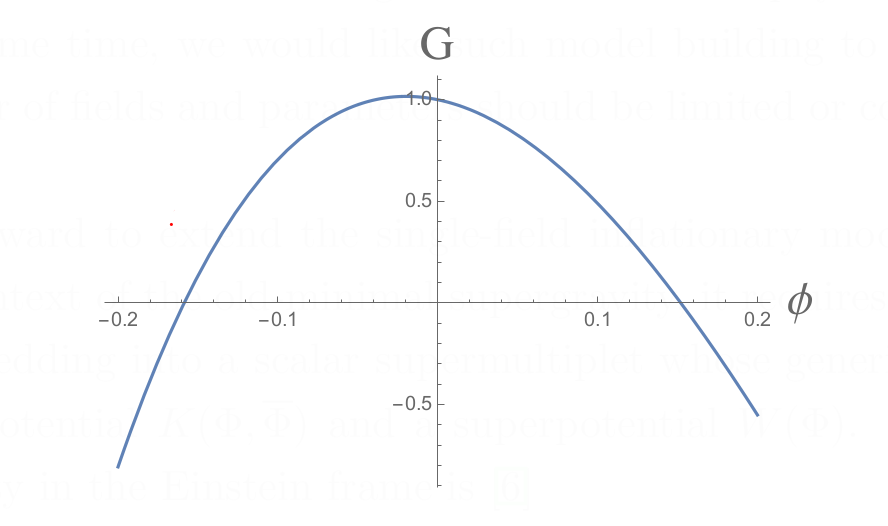
\includegraphics[width=5in]{Img/kinetic_coefficient_for_Phi.png}
  \caption{$\zeta=1$时,手征场$\Phi$的动能项系数与$\phi$的函数关系}\label{fig:kinetic-coefficient_for_Phi}
\end{figure}

从图$(\ref{fig:kinetic-coefficient_for_Phi})$可知,为了使$G>0$,$\phi$被限制在一
个有限的区间内。$\zeta$越大,$\phi$的取值区间越窄。因而在暴涨期间,标量场$\phi$的影响可以忽略,暴涨势近似为暴涨场$\chi$的函数,K\"ahler势中四次方项的调节作用
在这里清晰地体现出来了。当超势为
\begin{equation}
  W = \frac{1}{\sqrt{2}} f(-\sqrt{2}i\Phi),
\end{equation}
其中,$f$为实函数,沿暴涨场方向的暴涨势为
\begin{equation}
  V\simeq {\left[f_{,\chi}(\chi)\right]}^2.
\end{equation}
暴涨结束后,场朝着全局最小值滚去,最终得到一个超对称闵可夫斯基真空。这种情况对一
大类的超势都成立,同时也期望能在此基础上通过对K\"ahler势作一个微小的修正,能够抬升真空能得到德$\cdot$西特真空。然而no-go定理\citep{kallosh2014analytic}告诉我们对K\"ahler势和超势作一个无穷小修改,无法将具有超对称的闵可夫斯基真空连续地变化到德$\cdot$西特真空。举一个例子,当超势取如下形式时
\begin{equation}
  W=m(c\Phi+1),  
\end{equation}
\begin{figure}
  \centering
  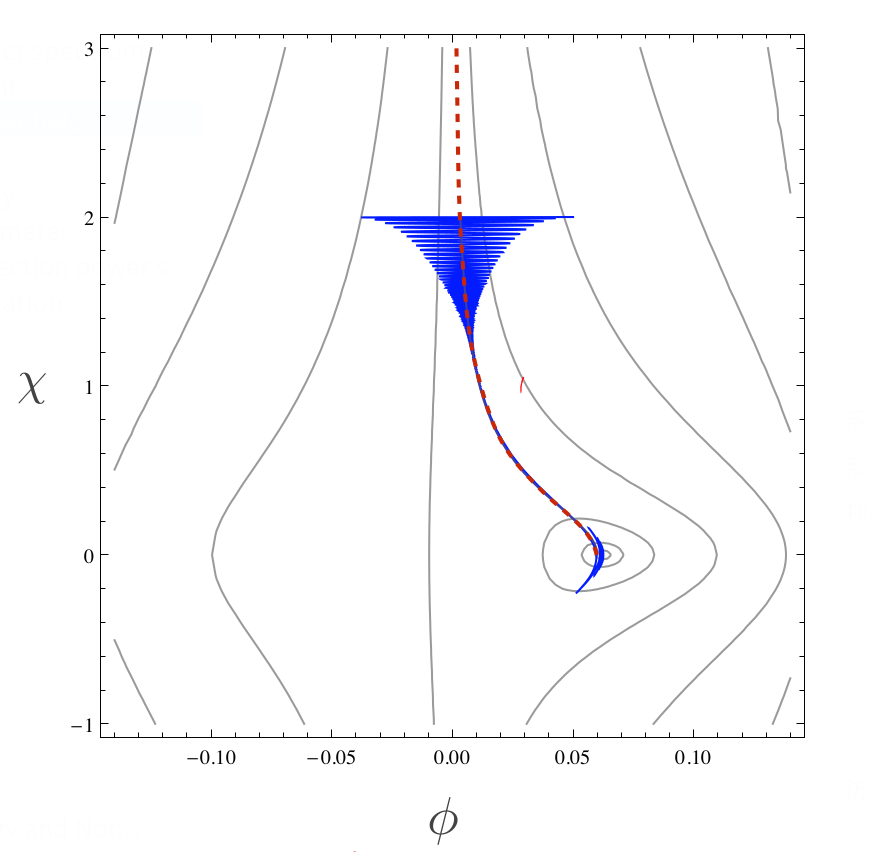
\includegraphics[width=5in]{Img/potential-for-linear-superpotential.png}
  \caption{蓝实线为数值计算得到的暴涨场的演化过程,红虚线为有效暴涨势的绝热近似。黑实线为暴涨势$V(\phi(\chi),
  \chi)$的对数等高线。当暴涨场靠近吸引子解前以及暴涨结束后都有一个震荡阶段。}\label{fig:potential-for-linear-superpotential}
\end{figure}
$c$和$d$为实参数,在$\phi=0$方向上暴涨势为
\begin{equation}
  V(\phi=0,\ \chi)=m^2c(c-2\sqrt{3}).
\end{equation}
显然参数$c$的大小将决定暴涨势大于零还是小于零。更具体的分析会发现,暴涨发生的过程并不完全在$\phi=0$方向。从图$(\ref{fig:potential-for-linear-superpotential})$中可以
看到,暴涨结束后得到的是一个超对称破缺的闵可夫斯基真空。通过对参数$c$进行微小的调节就能得到预期的德$\cdot$西特宇宙,$V_0\sim
10^{-120}$。但是代价为引起了强超对称破缺,得到的引力微子质量$m_{3/2}$比通常
理论预期的TeV量级高出多个量级。当考虑到粒子物理标准模型的时候,暴涨结束后是否
恢复超对称性是一件很重要的事情。例如
\citep{endo2006moduli,nakamura2006gravitino,kawasaki2006gravitino,kawasaki2006gravitino-overproduction,asaka2006gravitinos}
指出当真空超对称性破缺时,早期宇宙中从暴涨场衰变得到的引力微子数目会增多,
而这将引起灾难。另外\citep{degrassi2012higgs}中指出如果超对称破缺的能标过高,
电弱真空会遇到稳定性问题。

为了规避上述困难,同时在不破坏no-go定理的前提下,有两种方法既能抬升真空势能
得到德$\cdot$西特真空又能避免大的超对称破缺。一是引入额外的手征多态
(Polonyi场),并且对其施加强约束尽可能降低其对宇宙演化的影响
\citep{dudas2013strong}。另一个方法是引入零幂手征超场
\citep{ferrara2014cosmology,kallosh2015inflation,dall2014sgoldstino,kallosh2015inflation-de-sitter,linde2015does},
并且能从弦论中找到理论解释\citep{kallosh2014emergence}。

沿着这个思路,\citep{ketov2016susy}讨论了暴涨结束后恢复超对称性的条件,以及通过添加一个满足零幂条件$S^2=0$的Polonyi超场作为超对称破缺场$S$来控制超对称破缺的能标。


仍然考虑带有平移对称性的K\"ahler势\citep{ketov2016susy}
\begin{align}
    K=ic(\Phi-\bar\Phi)-\frac{1}{2}{(\Phi-\bar\Phi)}^2-\frac{\zeta}{4}{(\Phi-\bar\Phi)}^4,
\end{align}
其中$c$和$\zeta$为实参数。暴涨场取为手征超场$\Phi=(\phi+i\chi)/\sqrt{2}$的实部分量$\phi$。只要四次方项$\frac{\zeta}{4}{(\Phi-\bar\Phi)}^4$中的$\zeta$取得足够大,则暴涨场$\phi$在暴涨期间,场$\chi$的期望为$\langle\chi\rangle\approx0$。

参考了racetrack模型\citep{krasnikov1987supersymmetry,escoda2003saltatory,blanco2005racetrack}和其他模型\citep{ketov2016susy},我们选取如下形式的超势
\begin{align}
    W=a_0(1+a_1e^{-b_1\Phi}+a_2e^{-b_2\Phi}+a_3e^{-b_3\Phi}).
\end{align}

如果我们在宇宙学常数为零的真空中恢复了真空的超对称性
(关于真空中的超对称破缺问题的讨论请参考文献
\citep{gao2015inflection}),则F-term和暴涨势V在$\Phi=0$处应当都为零,
即$D_{\Phi}W=0$,$V=0$,这要求超势W满足约束条件
\begin{align}\label{eq:sp_constrain}
    W=\partial_{\Phi}W=0.
\end{align}
求解约束条件 (\ref{eq:sp_constrain}) 可以消去参数$a_1$和$a_2$
\begin{align}
    a_1\rightarrow \frac{b_2+a_3b_2-a_3b_3}{b_1-b_2},\qquad 
    a_2\rightarrow \frac{-b_1-a_3b_1+a_3b_3}{b_1-b_2}.
\end{align}
将K\"ahler势和超势代入到公式
\begin{align}
    V=e^{K}\lbrack
    D_{\Phi_i}W{(K^{-1})}^{ij^{*}}D_{\Phi^{*}_j}W^{*} - 3|W|^2\rbrack,
\end{align}
中,可以得到标量势$V(\phi)$。其中,
\begin{align}
    D_{\Phi}W=\partial_{\Phi}W + {(\partial_{\Phi}K)}W.
\end{align}
以及K\"ahler度规的逆,
\begin{align}
    K^{ij*} = \frac{\partial^2K}{\partial\Phi_i\partial\Phi^{*}_j}.
\end{align}

当在参数空间中选取某组参数如
\begin{align}\label{eq:parameters}
    a_0 = 4.35\times 10^{-6},
    a_3 = 7\times 10^{-8},
    b_1 = 3.05,
    b_2 = 6.3868164,
    b_3 = -4.4,
    c = 2.8.
\end{align}
时,标量势$V(\phi)$有两个近反射点,如图\ref{fig:potential}中所示。
场取较大值处的拐点给出与当前CMB数据相一致的标量功率谱的谱指标和张标比,
较小值处的拐点可以使标量扰动的功率谱产生一个尖峰从而生成原初黑洞。
\begin{figure}[!htbp]
    \centering
    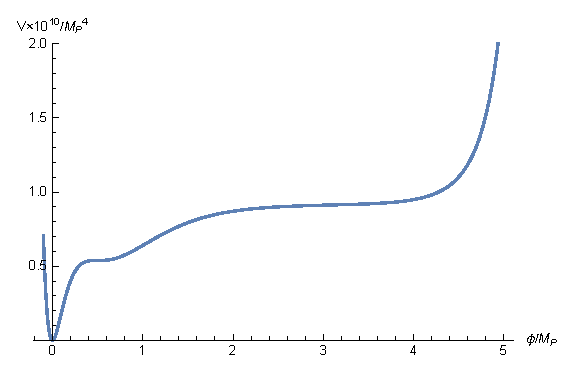
\includegraphics[width=5in]{Img/potential.eps}
    \caption{双拐点标量势$V(\phi)$}\label{fig:potential}
\end{figure}

在FLRW背景以及单场慢滚框架下,基于势能的慢滚参数$\epsilon_V$和$\eta_V$为
\begin{align}
  \epsilon_V &= \frac{1}{2}{\left(\frac{V_{,\phi}}{V(\phi)}\right)}^2, \\
  \eta_V &= \frac{V_{,\phi \phi}}{V(\phi)}.
\end{align}

由于在拐点附近暴涨势变得极端平坦,因此慢滚近似不再适用\citep{dimopoulos2017ultra,germani2017primordial},代之以极端慢滚暴涨。此时为了更精确地求解暴涨过程,势能慢滚参数需要替换为哈勃慢滚参数\citep{schwarz2001higher,leach2002cosmological,schwarz2004primordial},
\begin{align}
    \epsilon_H &= -\frac{\dot{H}}{H^2}, \\
    \eta_H &= -\frac{\ddot{H}}{2H\dot{H}}=\epsilon_H-\frac{1}{2}\frac{d \ln\epsilon_H}{dN_e}, \\
    \xi_H &=
    \frac{\dddot{H}}{2H^2\dot{H}}-2\eta^2_H=\epsilon_H\eta_H-\frac{d\eta_H}{dN_e},
\end{align}
其中,$N_e(t)$表示从视界穿过$k_{\star}$到暴涨结束期间的e-folding数,通常在取值在范围$50\sim60$之间。

标量扰动谱指标及其跑动和张标比的领头阶可以用$\epsilon_H,\eta_H,\xi_H$来表示
\begin{align}
    n_s &= 1- 4\epsilon_H+2\eta_H, \\
    \alpha &= \frac{dn_s}{d\ln k}=10\epsilon_H\eta_H-8\epsilon_H^2-2\xi_H, \\
    r &= 16\epsilon_H.
\end{align}

在参数集 (\ref{eq:parameters})下,相应的数值结果为
\begin{align}
  n_s &= 0.9635,\\
  \alpha&=-0.00369,\\
  r&=0.00276,
\end{align}

当$k_{\star}=0.05Mpc^{-1}$时,在$68\%$的置信水平上与Planck
2018给出的对CMB的限制结果相一致\citep{akrami2018planck}
\begin{align}
  n_s &= 0.9640\pm 0.0043,\\
  \alpha &= -0.0071\pm 0.0068,\\
  r &< 0.079.
\end{align}

标量扰动的功率谱在慢滚暴涨模型通常用近似公式
\begin{equation}
  \label{eq:scalar-perturbation-power-spectrum}
  \mathcal{P}_{\mathcal{R}} = \frac{V}{24\pi^2 \epsilon_V}.
\end{equation}
计算得到。由于在拐点处,暴涨势导数为零,因此使用势能慢滚参数的功率谱近似公式在
拐点处产生无穷大,导致公式失效。因而
\citep{germani2017primordial,motohashi2017primordial}中采用了不同的近似公式,
由于哈勃慢滚参数在整个暴涨期间始终大于零,因此基于哈勃慢滚参数的近似功率谱公式
\begin{equation}
  \label{eq:scalar-perturbation-power-spectrum-hubble}
  \mathcal{P}_{\mathcal{R}} \simeq
  \frac{1}{8\pi^2}\frac{H^2}{\epsilon_H}.
\end{equation}
将会给出更准确的结果。不过仍然指出这种近似可能会导致对PBH的质量函数产生错误的
估计,因而 \citep{ballesteros2018primordial}中根据Mukhanov-Sasaki (MS)公式
\citep{sasaki1986large,mukhanov1988quantum}数值求解精确的功率谱。 
Mukhanov-Sasaki (MS)方程为
\begin{align}\label{eq:ms}
    \frac{d^2u_k}{d\eta^2}+\left(k^2-\frac{1}{z}\frac{d^2z}{d\eta^2}\right)u_k=0,
\end{align}
其中$\eta$为共形时间,$z\equiv\frac{a}{\mathcal{H}}\frac{d\phi}{d\eta}$。初值条件取为Bunch-Davies真空\citep{bunch1978quantum}
\begin{align}
    u_k\rightarrow\frac{e^{-ik\eta}}{\sqrt{2k}},\quad\text{as}\quad
    \frac{k}{aH}\rightarrow\infty.
\end{align}

出于数值求解的方便,我们将共形时间$\eta$替换为$N_e$,把MS方程重写为\citep{ballesteros2018primordial}
\begin{align}
    \frac{d^2u_k}{dN^2_e}+\left(1-\epsilon_H\right)\frac{du_k}{dN_2}+
    \lbrack\frac{k^2}{\mathcal{H}^2}+\left(1+\epsilon_H-\eta_H\right)\left(\eta_H-2\right)-\frac{d\left(\epsilon_H-\eta_H\right)}{dN_e}=0,
\end{align}
原初功率谱由下式给出
\begin{align}
    \mathcal{P_R}=\frac{k^3}{2\pi^2}\left\lvert\frac{u_k}{z}\right\rvert^2_{k\ll
    \mathcal{H}}.
\end{align}

图\ref{fig:pert}为MS方程\ref{eq:ms}基于参数集\ref{eq:parameters}的数值结果。从图中可以发现功率谱在小尺度有一个高峰,在CMB的尺度上大约增长了7个数量级。这样大的一个密度扰动使得原初黑洞能够通过引力塌缩形成。

\begin{figure}[!htbp]
    \centering
    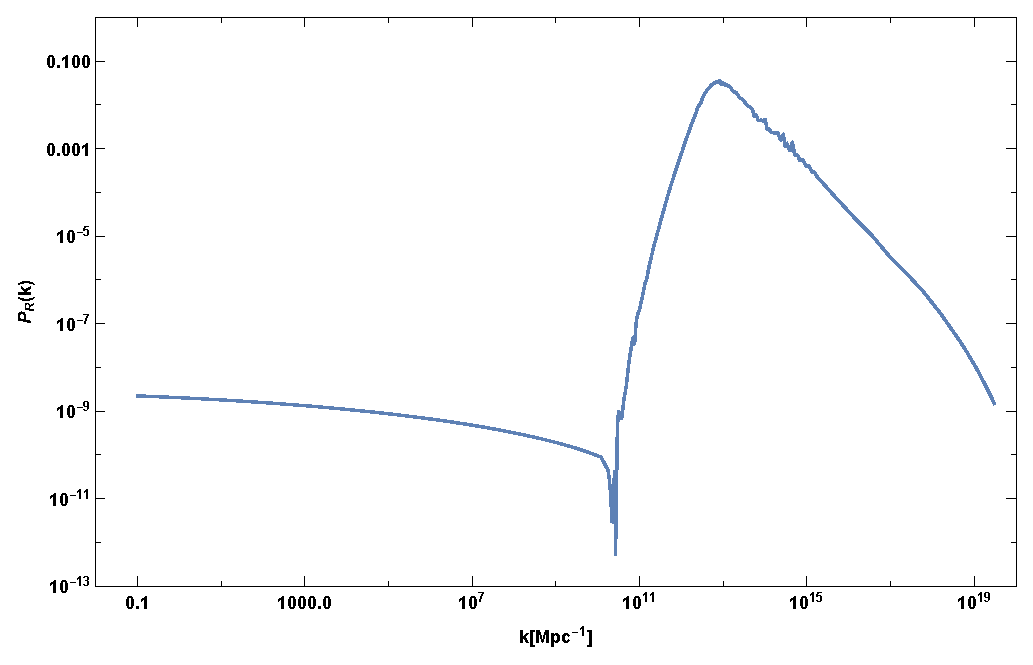
\includegraphics[width=5in]{Img/pert.eps}
    \caption{双拐点暴涨模型预测的标量扰动的原初功率谱$\mathcal{P_R}$}\label{fig:pert}
\end{figure}
